
%(BEGIN_QUESTION)
% Copyright 2006, Tony R. Kuphaldt, released under the Creative Commons Attribution License (v 1.0)
% This means you may do almost anything with this work of mine, so long as you give me proper credit

Identifiser tilhørende strømningskarakteristikk ({\it linear}, {\it equal percentage} eller {\it quick opening}) for hver globeventil som vises her:

$$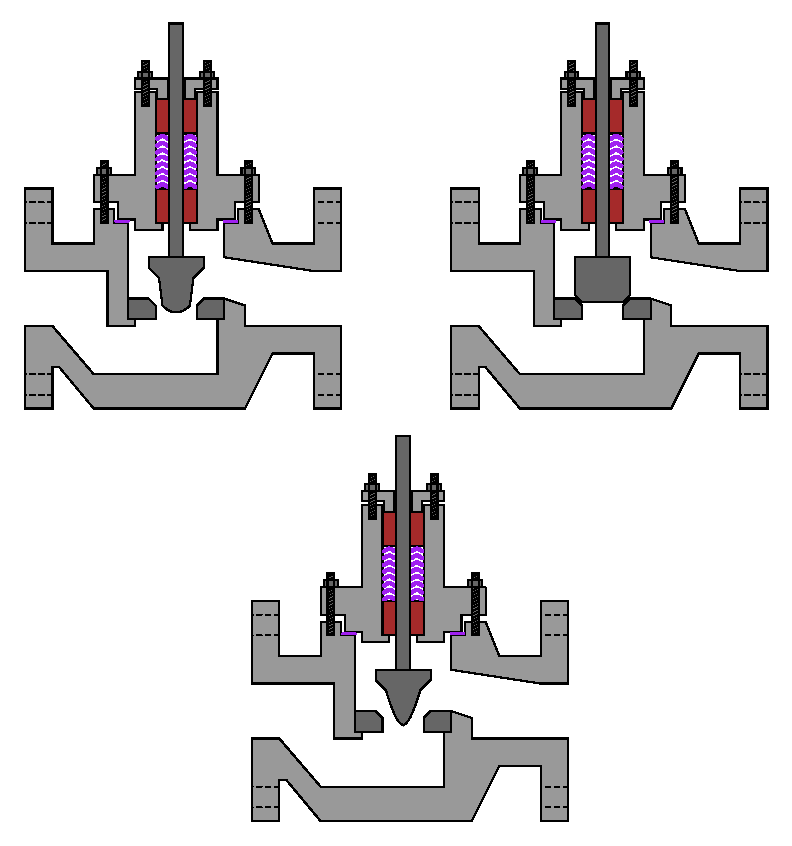
\includegraphics[width=15.5cm]{i01382x01.eps}$$

\vfil \eject

Identifiser deretter tilhørende strømningskarakteristikk ({\it linear}, {\it equal percentage} eller {\it quick opening}) for hver roterende kuleventil som vises her:

$$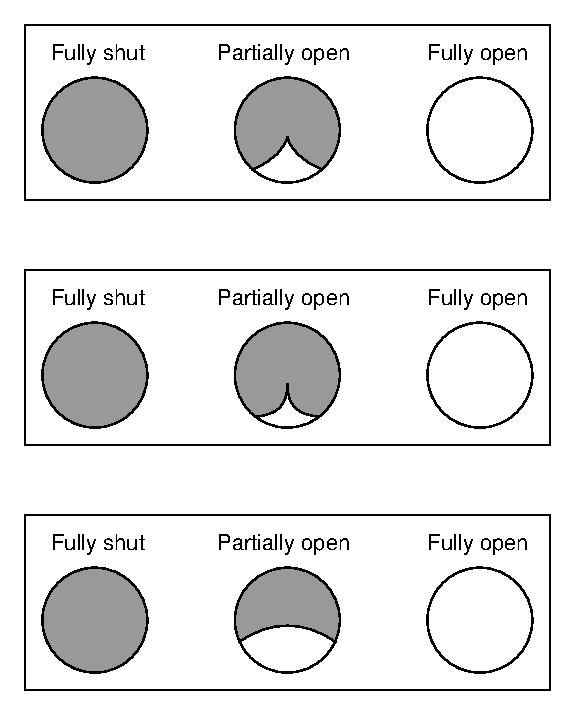
\includegraphics[width=15.5cm]{i01382x04.eps}$$

\vskip 20pt \vbox{\hrule \hbox{\strut \vrule{} {\bf Forslag til sokratisk diskusjon} \vrule} \hrule}

\begin{itemize}
\item{} Det viktigste med svaret ditt på denne oppgaven, som vanlig, er {\it hvordan} og {\it hvorfor} du kom fram til valgene. Forklar hvordan du kan avgjøre hver ventils karakteristikk bare ut fra utseendet på trim-tverrsnittene.
\end{itemize}

\underbar{file i01382}
%(END_QUESTION)





%(BEGIN_ANSWER)

%(END_ANSWER)





%(BEGIN_NOTES)

Å identifisere lineær, equal-percentage og quick-opening trim er relativt enkelt når de tre trimtypene står side om side for sammenligning. Jeg liker å kalle dette ``Gullhår-metoden'': å finne riktig type ved å sammenligne relative former mot hverandre. Lineær blir trimformen som ligger ``mellom'' de to ytterpunktene equal-percentage og quick-opening.

$$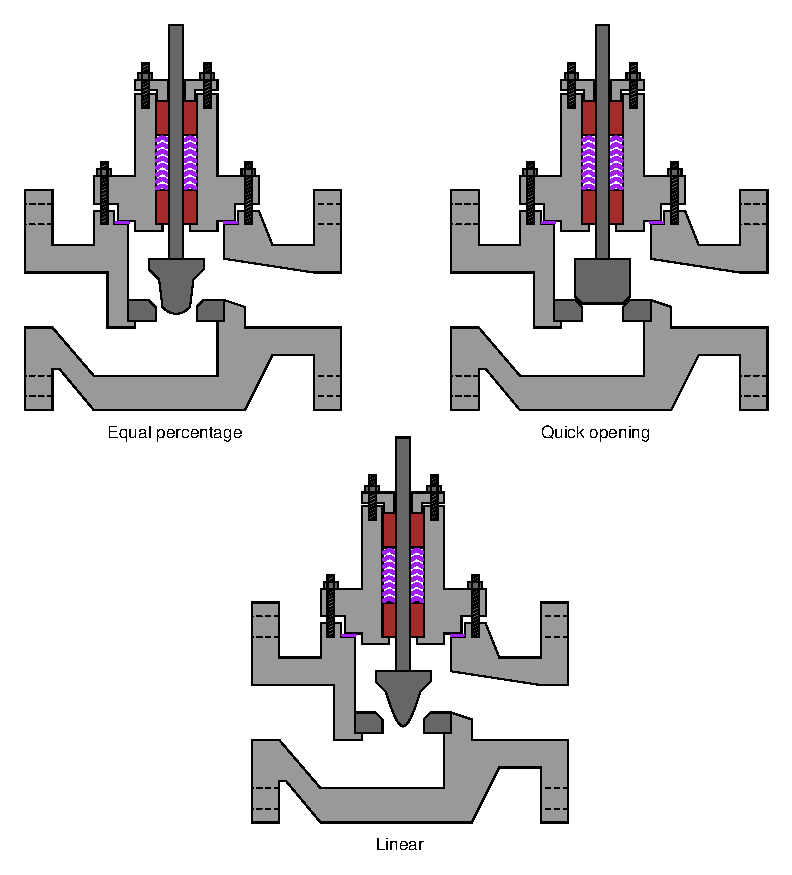
\includegraphics[width=15.5cm]{i01382x02.eps}$$

Quick-opening-ventilen bør være tydelig: den åpner raskt når pluggen løftes fra setet, fordi pluggen faktisk ikke går ned i setets ``hals'' slik de andre trimtypene gjør.

\vskip 10pt

Den nederste ventilen er {\it linear}, med en nesten perfekt konisk plugg som går inn gjennom setets hals. Dette gir en $C_v$ som varierer lineært med pluggvandring.

\vskip 10pt

{\it Equal percentage}-ventilen er øverst til venstre. Pluggen har brattere (mer vertikal) stigning enn lineær-pluggen, noe som gjør at $C_v$ øker saktere i starten. Mot bunnen blir pluggen flatere, og dermed øker $C_v$ raskere mot slutten av pluggvandringen.

\vskip 10pt

\filbreak

$$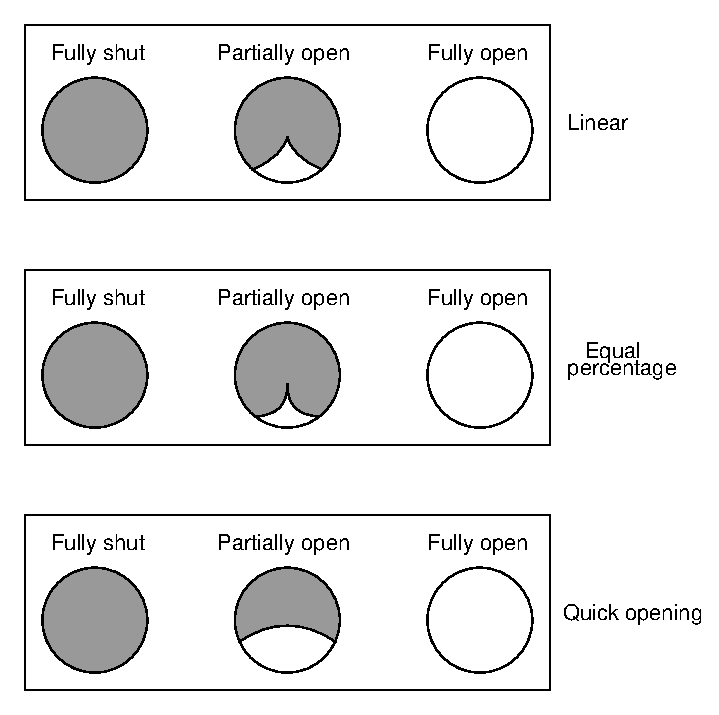
\includegraphics[width=15.5cm]{i01382x05.eps}$$









\vfil \eject

\noindent
{\bf Oppsummeringsquiz:}

Velg globeventiltrim med {\it quick-opening}-karakteristikk:

$$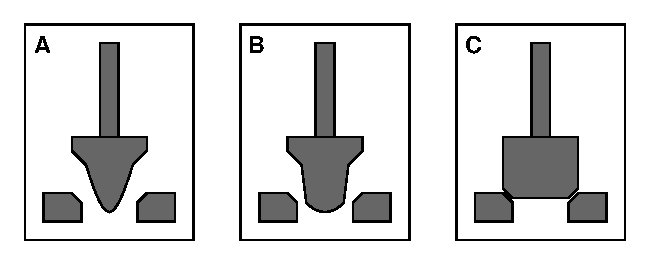
\includegraphics[width=15.5cm]{i01382x03.eps}$$










\vfil \eject

\noindent
{\bf Oppsummeringsquiz:}

Velg globeventiltrim med {\it equal-percentage}-karakteristikk:

$$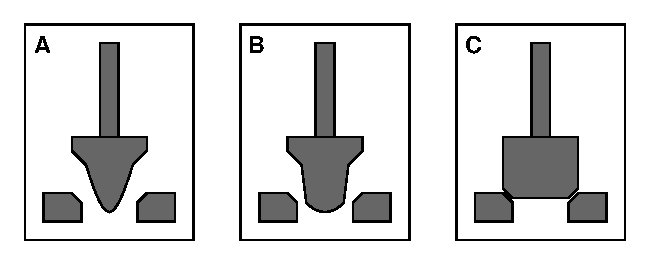
\includegraphics[width=15.5cm]{i01382x03.eps}$$










\vfil \eject

\noindent
{\bf Oppsummeringsquiz:}

Velg globeventiltrim med {\it linear}-karakteristikk:

$$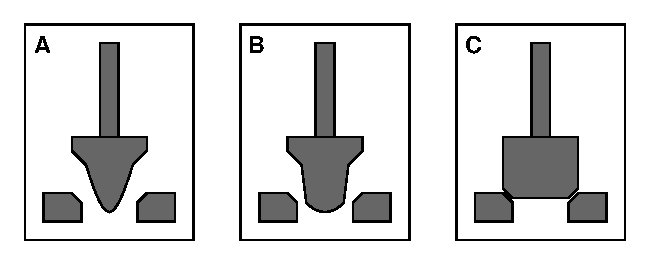
\includegraphics[width=15.5cm]{i01382x03.eps}$$


%INDEX% Final Control Elements, valve: characterization

%(END_NOTES)

